\documentclass{standalone}
\usepackage{tikz}
\usepackage{ctex,siunitx}
\setCJKmainfont{Noto Serif CJK SC}
\usepackage{tkz-euclide}
\usepackage{amsmath}
\usetikzlibrary{patterns, calc}
\usetikzlibrary {decorations.pathmorphing, decorations.pathreplacing, decorations.shapes,}

\begin{document}
\small
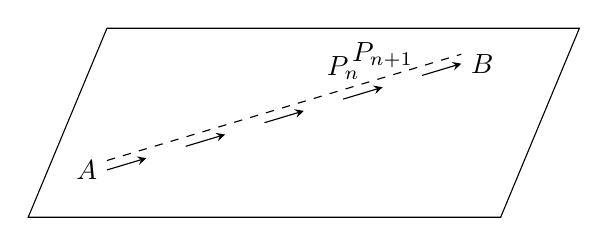
\begin{tikzpicture}[>=stealth,yscale=0.6]
  \tkzSetUpPoint[fill=black]
  % \useasboundingbox(-1,-0.75)rectangle(3.7,1.4);
	\draw(1,4)--(7,4)--(6,0)--(0,0)--(1,4);
	\draw[->](1,1)node[left]{$A$}--(1.5,1.25);
	\draw[->](2,1.5)--(2.5,1.75);
	\draw[->](3,2)--(3.5,2.25);
	\draw[->](4,2.5)--(4.5,2.75);
	\draw[->](5,3)--(5.5,3.25)node[right]{$B$};
	\draw[dashed](1,1.2)--(5.5,3.45);
  \node at (4,2.7)[above]{$P_n$};
  \node at (4.5,2.95)[above]{$P_{n+1}$};
\end{tikzpicture}
\end{document}